\section{Neural network architecture and training}
Each MHCflurry is a feed-forward neural network containing (1) an embedding layer which transforms amino acids to learned vector representations, (2) a single hidden layer, (3) a sigmoidal scalar output. We map IC50 concentrations onto a regression targets between 0.0 and 1.0 using the same scheme as NetMHC, $y = 1.0 - max(1.0, log_{50000}(IC50))$.

%% \begin{figure}[h]
%% \centering
%% 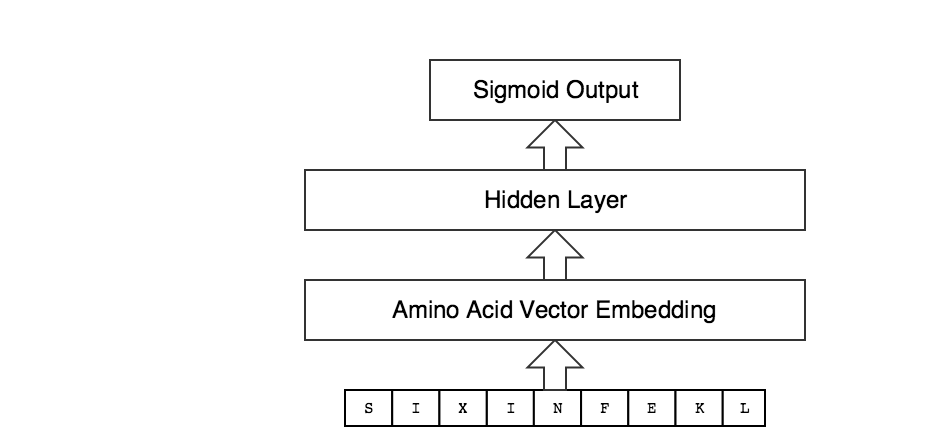
\includegraphics[scale=0.25]{figures/mhcflurry-gliffy-network.png}
%% \caption{MHCflurry architecture}
%% \label{fig:architecture}
%% \end{figure}

Like the NetMHC family of predictors~\cite{lundegaard2008accurate}, MHCflurry uses fixed length 9mer inputs which requires peptides of other lengths to be transformed into multiple 9mers. Shorter peptides are mapped onto 9mer query peptides by introducing a sentinel ``X'' at every possible position, whereas longer peptides are cut into multiple 9mers by removing consecutive stretches of residues. The predicted affinity for a non-9mer peptide is the geometric mean of the predictions for the generated 9mers. When $n$ training samples derive from a single non-9mer sequence then their weights are adjusted to $1/n$. 

For each allele, we train a MHCflurry model using the measured peptide affinities for the allele and the values imputed by MICE based on other alleles in the training set. As training progresses, we place quadratically decreasing weight on the imputed values.

A randomly generated peptide is unlikely to bind a given MHC strongly, but a data acquisition bias toward strong binders in the training set can lead models to assign a high affinity to most peptide. As a form of regularization, we augment the training set at each epoch to include random peptides with affinity set to be maximally weak. The number of random negative peptides is 20\% of the training size (without imputation). At each training epoch, a fresh set of random peptides is generated.

Three-fold cross validation on the training set was used to select the hyper-parameters. The model selected used 32 output dimensions for the amino acid vector embedding, a hidden layer size of 64, a dropout rate\cite{Srivastava2014} of 50\%, and 250 training epochs. These hyper-parameters achieved reasonable performance across alleles, but it's likely that performance could be slightly improved by setting the hyper-parameters separately for each allele.